\documentclass[main.tex]{subfiles}
\newcommand\chapterlabel{Ch-kinetics}
\setcounter{figurenewcounter}{0}

\chapterpicture{../{\chapterlabel}/figure1}\chapterpicturelabel{PxFuel}

\begin{document}
\linenumbers
%\setcounter{chapter}{5}
  
\chapter[Chemical kinetics]{Chemical kinetics}
%\label{ch:atoms}

%
%      \begin{marginfigure}
%      \begin{tikzpicture} \node (a) at (0,0) {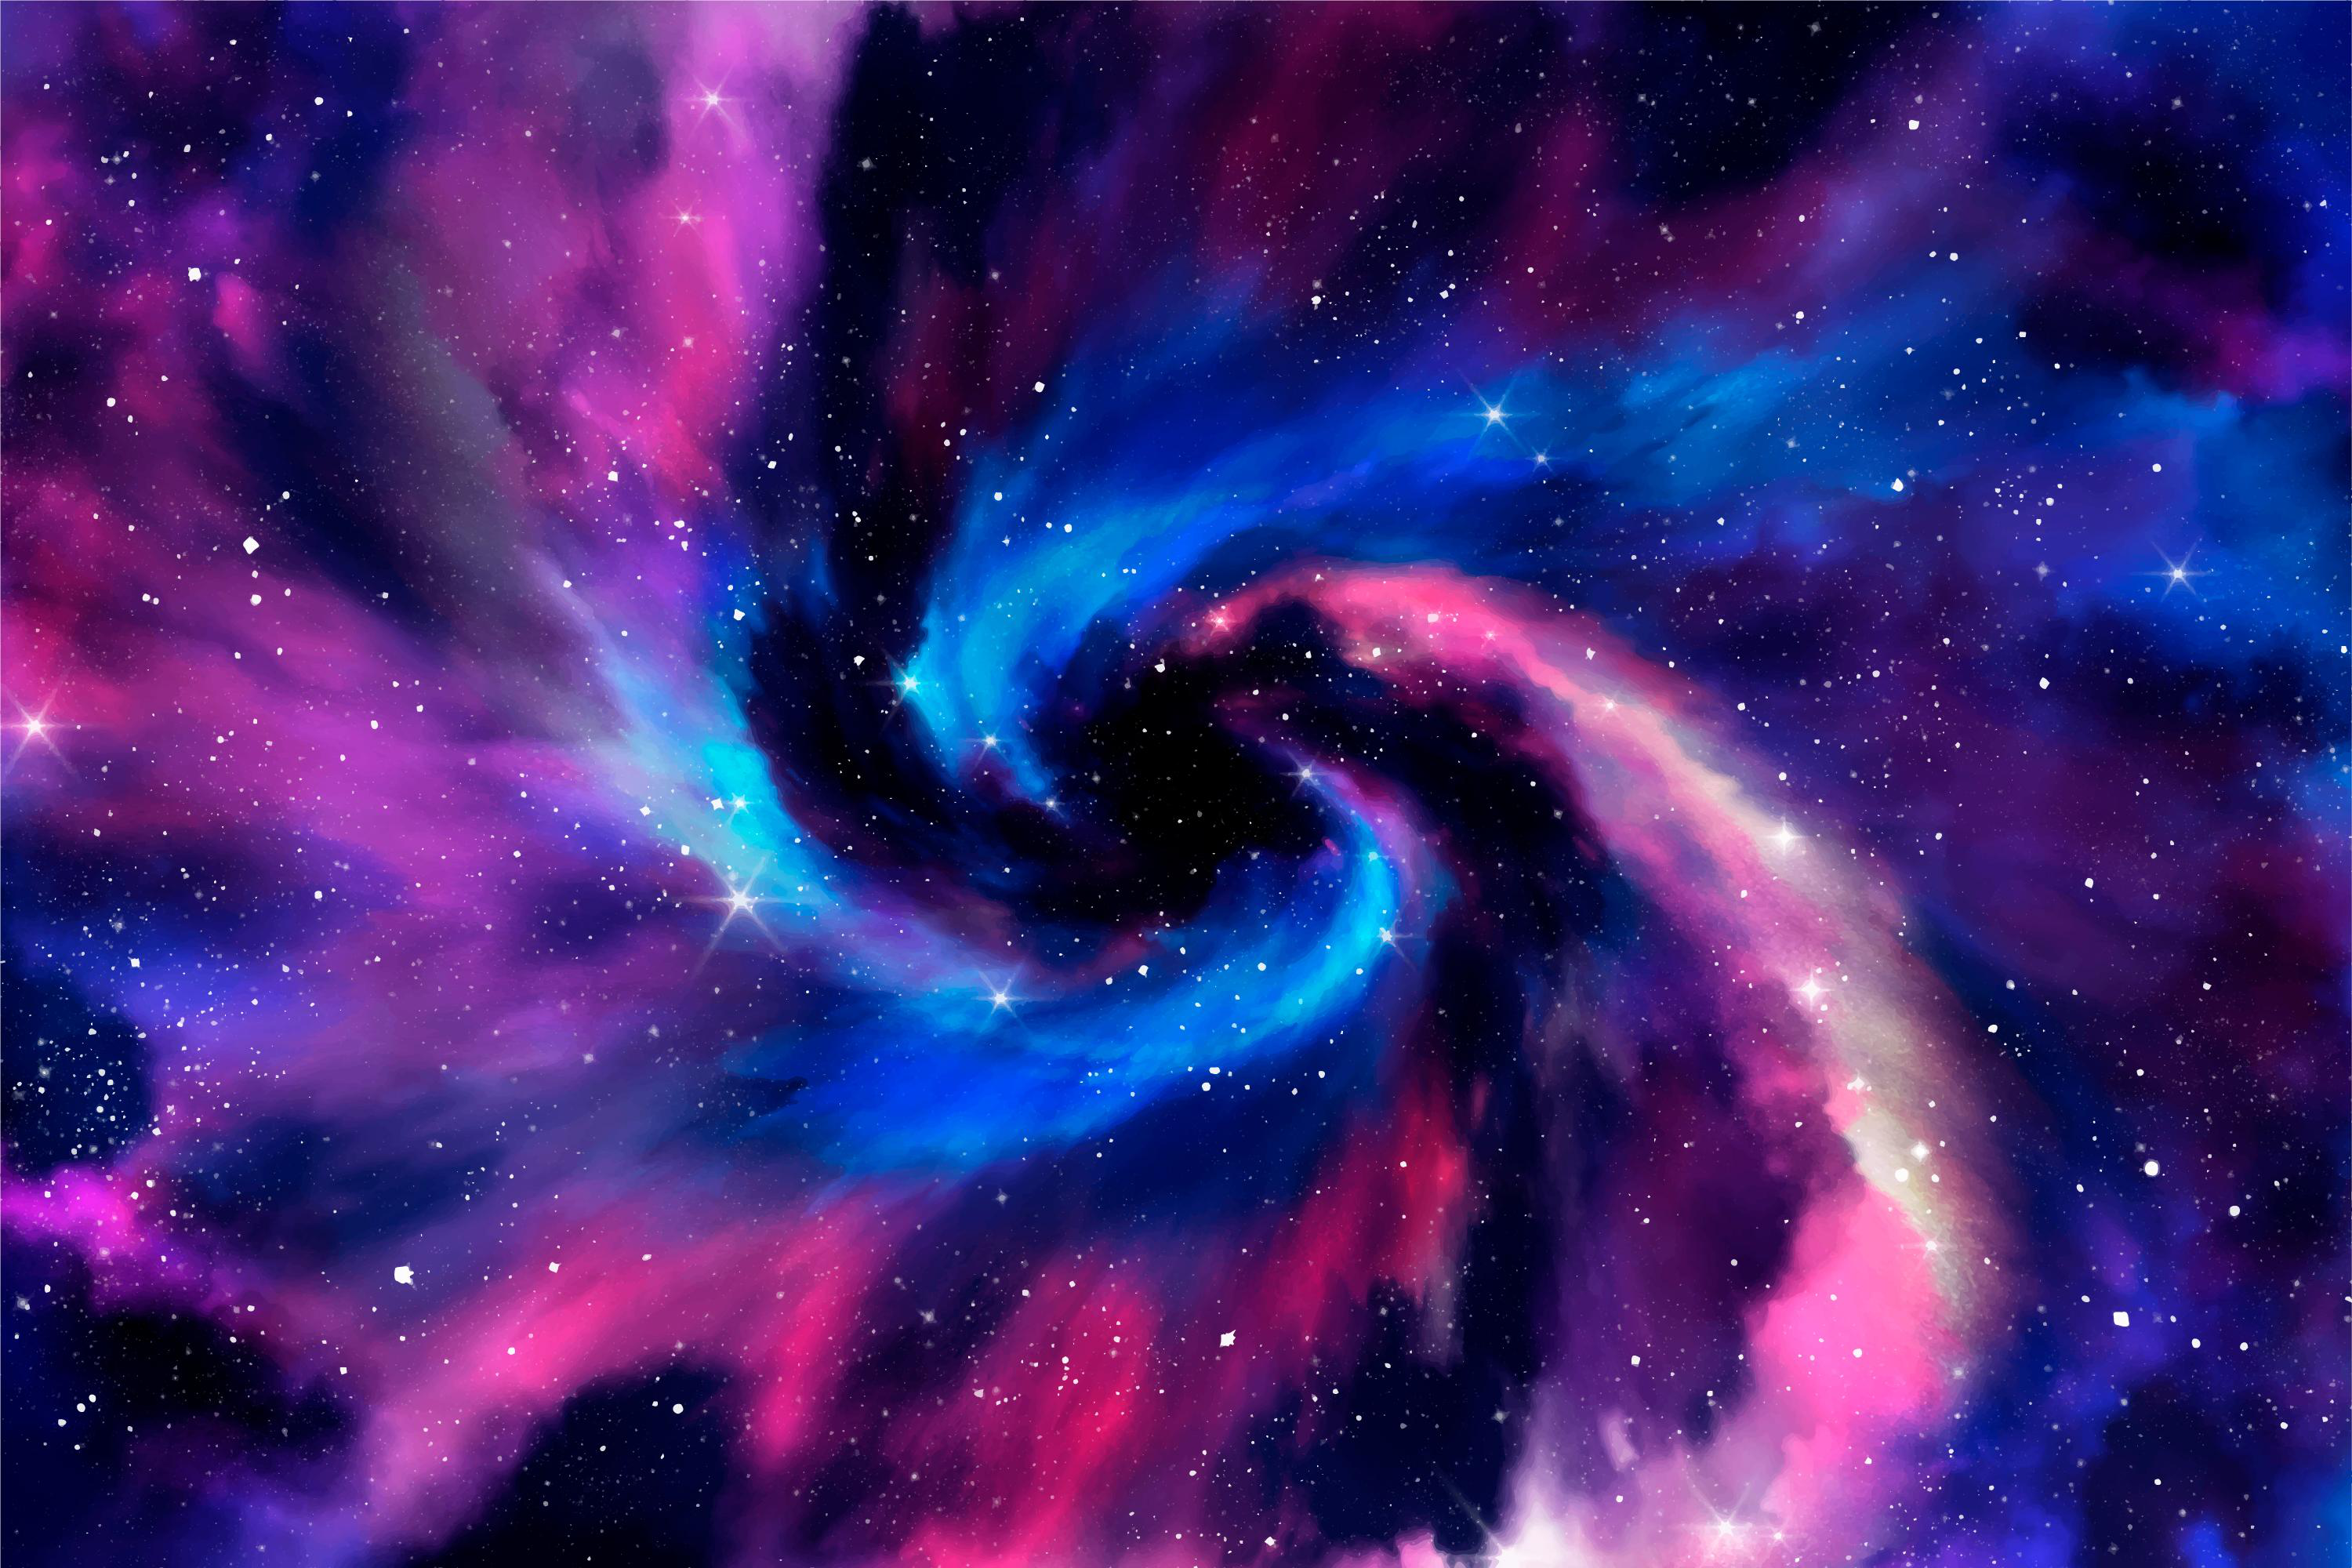
\includegraphics[width=4cm]{../Ch-kinetics/figure1}} node[rotate=90, font=\tiny] at ([yshift=.5cm,xshift=.1cm]a.south east) {\textsuperscript{\textcopyright} PxFuel} ;
%\end{tikzpicture}
%\end{marginfigure}


\lettrine[lines=4]{\color{black!45}T}{he} rate at which a chemical reaction occurs is a critical parameter at an industrial and laboratory-level as the faster the speed the sooner one can commercialize or sell a given chemical product. Slow chemical reactions are, in general, less desirable as it takes more time for the reagents to react. On the other hand, too fast chemical reactions can also be less desirable. Think, for example, in an explosion in which gas and a spark quickly generate carbon dioxide with water and a lot of heat in a way that is not easy to control. This chapter deals with the rate of reactions. You will learn how to calculate what we call a rate law which is a mathematical formula that gives the numerical rate value. You will also learn the collision theory that explains the factors that affect the speed of chemical reactions. 
%\begin{marginfigure}%LEARNING GOALS BOX
%\begin{mytcbox}{GOALS}
%\begin{enumerate}[label=\protect\circled{\color{white}\arabic*}]
%\item Analyze a rate law
%\item Interconvert rates of reactants and products
%\item Obtain rate laws
%\item Compute activation energies
%\item Analyze energy profiles
%\end{enumerate}
%\end{mytcbox}
%\vspace{1cm}
%\begin{tcolorbox}[enhanced,colback=red!5!white,colframe=black!50!red,boxrule=1pt,
%  arc=0pt,outer arc=0pt,drop heavy lifted shadow]
%\faGears\ 
%\docenvdef{Discussion:} (a) \discussionKINETICSA (b) \discussionKINETICS \end{tcolorbox}
%\end{marginfigure}%LEARNING GOALS BOX



\section{Rate of reaction}
Some chemical reactions are fast such as the explosive reaction between cooking gas and oxygen, happening almost instantaneously. Other reactions are slow such as the rusting of iron, taking months to occur. Chemical kinetics is a chemistry discipline that studies the speed of chemical reactions and the factors that affect this measure. The overall goal here is to understand the factors that control the rate of reactions with the ultimate goal of maximizing the generation of products. This section covers the principles of reaction rates, defining two different types of rates, and showing how to interconvert rates of reaction.
\sloppy 
\begin{description}
\item[\docfilehook{Two different ways of defining the reaction rate}{}] 
When a chemical reaction proceeds, reactants decompose into products. Therefore, the concentration of reactants decreases with time as reactant molecules become products, and the concentration of products increases with time as products are being formed. This change in concentration with time is what we call reaction rate. There are two different ways of defining the rate of a reaction. We can define the average reaction rate $\overline{r}$ as the change in concentration with time or as an instantaneous rate $r$ when the time interval is very small (we call this derivative):
\begin{equation}
\boxed{\overline{r}=\frac{\Delta c}{\Delta t} 
\quad  \text{or }\quad 
 r=\lim\limits_{\Delta t \to 0}     \frac{\Delta c}{\Delta t}=\frac{d c}{d t}}
\label{\chapterlabel:equation1}
\end{equation}
Both types of rates are not numerically the same. The average rate is an average change in concentration between two different times. At the same time, the time interval for the average can be large or small.
Differently, the instantaneous rate is calculated as the slope in the concentration vs. time plot at a given time--using mathematical terms we call this the derivative. Instantaneous rates represent more accurately the changes in concentration happening in a reaction. For this reason, from now on, whenever we describe a reaction rate we will refer to the instantaneous rate.
\item[\docfilehook{Rate of appearance and disappearance}{}] 
At the beginning of a reaction, the molecules of reactants will be consumed while the molecules of products will form. There are three different ways to measure the reaction rate. We can measure the amount of reactants that disappear per unit of time and this would give you the rate of disappearance of a reactant. We can also measure the amount of products formed per unit of time and that would give you the rate of appearance of a  product. As a note, rates of disappearance are negative (as the molarity of reactants decreases with time) whereas rates of appearance are positive. Finally, we can measure the amount of reactants the interconvert into products and that would give you the overall rate of reaction, which is always a positive number. Overall, by measuring concentration changes of reactants and products we can compute three types of rates: rates of disappearance, rates of appearance, and rates of reaction.

    \stepcounter{figurenewcounter}   \refstepcounter{figure}  \label{Fig:{\chapterlabel}\thefigurenewcounter}
     \begin{center}
    \pgfkeys{tikz/.cd,
tangent length/.store in=\TangentLength,
tangent length=7mm,
normal length/.store in=\NormalLength,
normal length=7mm}
\tikzset{tangent/.style={red,thin},normal/.style={red,thin},
tangent at/.style={postaction={decorate,decoration={markings,
mark=at position #1 with {\draw[tangent,shift={(0,1.60em-1.6em)}, rotate=-0] (-2*\TangentLength,0) -- (0.4*\TangentLength,0)   -- ++ (-4.7em,-0.6em) -- cycle; \node[shift={(-2em,1em)}, red] (-\TangentLength,0) {$r$} node[shift={(-4.4em,.3em)}, red] (-\TangentLength,0) {\tiny $d$c} node[shift={(-2em,-.2em)}, red] (-\TangentLength,0) {\tiny $d$t};
\fill[tangent,shift={(0,1.60em-1.6em)}]  (-\TangentLength,0) circle (1pt);}}}},
%normal at/.style={postaction={decorate,decoration={markings,
%mark=at position #1 with {\draw[normal] (0,-\NormalLength) -- (0,\NormalLength);
%\fill[normal] (0,0) circle (2pt);}}}},
}
\begin{tikzpicture}
  \begin{axis}[
            axis lines=middle,
             enlargelimits=0.1,
            xmin=0,
            xmax=1.0,
            ymin=0.01,
            ymax=0.1,
            xtick=\empty,
            ytick=\empty,xtick distance=0.05,
            xlabel=$\text{time}$,
            ylabel=$c\text{, M}$,
            x label style={at={(axis description cs:0.5,-0.0)},anchor=north},
    y label style={at={(axis description cs:0.07,.4)},rotate=90,anchor=south},
             domain=\pgfkeysvalueof{/pgfplots/xmin}:(\pgfkeysvalueof{/pgfplots/xmax},
            tangent/.style={add node at x={#1}{},},
        ]
     	              
            \addplot [thick,draw=blue!75!black, tangent at/.list={ 0.8 }]{0.1*exp(-2.9*x)};
                         \addplot [blue!75!black, mark=*,  draw=none , samples=5 ]{0.1*exp(-2.9*x)};
	 \draw[red] (6.4em,6em+0.8em) --++(0em,-3.5em+0.1em)--++(6.1em,0em ) -- cycle ;
	 \node[shift={(8.5em,5.5em+0.7em)}] (0,0) {$\overline{r}$} node[shift={(5.5em,5em+0.7em)}] (0,0) {\tiny $\Delta c$} node[shift={(8.5em,2.0em+0.9em)}] (0,0) {\tiny $\Delta t$} node[green!75!black, shift={(23em,12em)}] (0,0) {\small Product} node[blue!75!black, shift={(23em,2em)}] (0,0) {\small Reactants} ; 
                \addplot  [thick,draw=green!75!black]{0.1*(1-exp(-2.9*x))};
	             \addplot  [green!75!black, mark=*,  draw=none , samples=5]{0.1*(1-exp(-2.9*x))}; 


        \end{axis}
     \begin{scope}[xshift =0em, yshift =0em]
\node[text width=12cm, fontscale=0.1, shift={(15em,-4em)}] at (-0em,-0em) { \begin{bf}\color{black}\bfseries\large Figure \ref{Fig:{\chapterlabel}\thefigurenewcounter} \end{bf} Change of the concentration of reactants and products with time showing the average and instantaneous velocity.  };
   \end{scope} 
\end{tikzpicture}\end{center}

Let us work on a sample reaction:
\begin{center}\ce{I^-_{(aq)} + OCl^-_{(aq)} -> Cl^-_{(aq)} + OI^-_{(aq)}}\end{center}
We can think of the rate of disappearance of \ce{I^-_{(aq)}} that should be written as:
\[r_{\ce{I^-}} =  \frac{d\ce{\text{[\ce{I^-}]}}}{d t}\]
Similarly, we have that the rate of appearance of \ce{Cl^-} is:
\[r_{\ce{Cl^-}} =  \frac{d\ce{\text{[\ce{Cl^-}]}}}{d t}\]
As chemical rates represent the change of concentration of a given reactant with time, the units for a chemical rate are M/s.
\item[\docfilehook{Relating rates of appearance and disappearance}{}] 
We can relate the rates of any two reactants or products in a chemical reaction and, at the same time, we can relate the rate of reaction with the rate of any product or reactant--remember there is a single rate of reaction and multiple rates of appearance and disappearance of products and reactants. For example, for the following reaction:
\begin{center}\ce{4NH3_{(g)} + 5O2_{(g)} -> 4NO_{(g)} + 6H2O_{(g)}}\end{center}
We can relate $r_{\ce{NH3}}$ and $r_{\ce{H2O}}$:
\[-\frac{1}{4}r_{\ce{NH3}}=+\frac{1}{6}r_{\ce{H2O}}\]
Overall, a negative sign should be included before the rate of any reactant and a positive sign before the rate of any product. You also need to divide by the stoichiometric coefficients of each reactant and product. Similarly, we can relate $r_{\ce{O2}}$ with the rate of reaction $r$:
\[-\frac{1}{5}r_{\ce{O2}}= r \]
For a general equation such as:
\begin{center}\ce{aA + bB -> cC + dD}\end{center}
we have that the general relationship between any rate and the overall reaction rate is:
\begin{equation}
\boxed{r=-\frac{1}{a}r_A=-\frac{1}{b}r_B=+\frac{1}{c}r_C=+\frac{1}{d}r_D  }
\label{\chapterlabel:equation2}
\end{equation}

\end{description}


  \import{../\chapterlabel/problems/}{SampleProblem1}





\vspace{3cm}
\begin{fullwidth}
\stepcounter{figurenewcounter}   \refstepcounter{figure}  \label{Fig:{\chapterlabel}\thefigurenewcounter}
     \begin{minipage}[b]{1.0\linewidth}\resizebox{0.9\textwidth}{!}{
\begin{tikzpicture}
 \begin{scope}[rotate=00, shift={(0em,0em)}] 
\draw[  black , very thick ]  (0.0,0.0) to (10.0em,0.0)    to  (10.0em,10.0em)  to  (0em,10.0em) --cycle  ;
\node [ fontscale=0.1, pos=0.9,shift={(5em,-1.0em)}] {0 min}   ;
\shade[ball color=green!70!white] (1em, 1em) circle (.2cm);\shade[ball color=green!70!white] (3em, 2.5em) circle (.2cm);\shade[ball color=green!70!white] (5em, 3.5em) circle (.2cm);\shade[ball color=green!70!white] (5em, 1.em) circle (.2cm);\shade[ball color=green!70!white] (8em, 2.em) circle (.2cm);\shade[ball color=green!70!white] (1em, 7em) circle (.2cm);\shade[ball color=green!70!white] (4em, 6em) circle (.2cm);\shade[ball color=green!70!white] (8em, 7em) circle (.2cm);\shade[ball color=green!70!white] (5em, 9em) circle (.2cm);
\end{scope}
 \begin{scope}[rotate=00, shift={(11em,0em)}] 
\draw[  black , very thick ]  (0.0,0.0) to (10.0em,0.0)    to  (10.0em,10.0em)  to  (0em,10.0em) --cycle  ;
\node [ fontscale=0.1, pos=0.9,shift={(5em,-1.0em)}] {5 min}   ;
\shade[ball color=red!70!white] (1em, 1em) circle (.2cm);\shade[ball color=green!70!white] (3em, 2.5em) circle (.2cm);\shade[ball color=green!70!white] (5em, 3.5em) circle (.2cm);\shade[ball color=green!70!white] (5em, 1.em) circle (.2cm);\shade[ball color=green!70!white] (8em, 2.em) circle (.2cm);\shade[ball color=green!70!white] (1em, 7em) circle (.2cm);\shade[ball color=green!70!white] (4em, 6em) circle (.2cm);\shade[ball color=green!70!white] (8em, 7em) circle (.2cm);\shade[ball color=green!70!white] (5em, 9em) circle (.2cm);
\end{scope}
 \begin{scope}[rotate=00, shift={(22em,0em)}] 
\draw[  black , very thick ]  (0.0,0.0) to (10.0em,0.0)    to  (10.0em,10.0em)  to  (0em,10.0em) --cycle  ;
\node [ fontscale=0.1, pos=0.9,shift={(5em,-1.0em)}] {10 min}   ;
\shade[ball color=red!70!white] (1em, 1em) circle (.2cm);\shade[ball color=green!70!white] (3em, 2.5em) circle (.2cm);\shade[ball color=green!70!white] (5em, 3.5em) circle (.2cm);\shade[ball color=green!70!white] (5em, 1.em) circle (.2cm);\shade[ball color=red!70!white] (8em, 2.em) circle (.2cm);\shade[ball color=green!70!white] (1em, 7em) circle (.2cm);\shade[ball color=red!70!white] (4em, 6em) circle (.2cm);\shade[ball color=green!70!white] (8em, 7em) circle (.2cm);\shade[ball color=green!70!white] (5em, 9em) circle (.2cm);
\end{scope}
 \begin{scope}[rotate=00, shift={(39em,0em)}] 
\draw[  black , very thick ]  (0.0,0.0) to (10.0em,0.0)    to  (10.0em,10.0em)  to  (0em,10.0em) --cycle  ;
\node [ fontscale=0.1, pos=0.9,shift={(5em,-1.0em)}] {500 min}   ;
\shade[ball color=red!70!white] (1em, 1em) circle (.2cm);\shade[ball color=red!70!white] (3em, 2.5em) circle (.2cm);\shade[ball color=green!70!white] (5em, 3.5em) circle (.2cm);\shade[ball color=red!70!white] (5em, 1.em) circle (.2cm);\shade[ball color=red!70!white] (8em, 2.em) circle (.2cm);\shade[ball color=red!70!white] (1em, 7em) circle (.2cm);\shade[ball color=red!70!white] (4em, 6em) circle (.2cm);\shade[ball color=green!70!white] (8em, 7em) circle (.2cm);\shade[ball color=green!70!white] (5em, 9em) circle (.2cm);
\node [ fontscale=0.1,  shift={(-4em,6em)}] {$\dots$}   ;
\end{scope}


 \begin{scope}[rotate=00, shift={(0em,-15em)}] 
\draw[  black , very thick ]  (0.0,0.0) to (10.0em,0.0)    to  (10.0em,10.0em)  to  (0em,10.0em) --cycle  ;
\node [ fontscale=0.1, pos=0.9,shift={(5em,-1.0em)}] {0 min}   ;
\shade[ball color=green!70!white] (1em, 1em) circle (.2cm);\shade[ball color=green!70!white] (3em, 2.5em) circle (.2cm);\shade[ball color=green!70!white] (5em, 3.5em) circle (.2cm);\shade[ball color=green!70!white] (5em, 1.em) circle (.2cm);\shade[ball color=green!70!white] (8em, 2.em) circle (.2cm);\shade[ball color=green!70!white] (1em, 7em) circle (.2cm);\shade[ball color=green!70!white] (4em, 6em) circle (.2cm);\shade[ball color=green!70!white] (8em, 7em) circle (.2cm);\shade[ball color=green!70!white] (5em, 9em) circle (.2cm);
\end{scope}
 \begin{scope}[rotate=00, shift={(11em,-15em)}] 
\draw[  black , very thick ]  (0.0,0.0) to (10.0em,0.0)    to  (10.0em,10.0em)  to  (0em,10.0em) --cycle  ;
\node [ fontscale=0.1, pos=0.9,shift={(5em,-1.0em)}] {5 min}   ;
\shade[ball color=red!70!white] (1em, 1em) circle (.2cm);\shade[ball color=red!70!white] (3em, 2.5em) circle (.2cm);\shade[ball color=green!70!white] (5em, 3.5em) circle (.2cm);\shade[ball color=green!70!white] (5em, 1.em) circle (.2cm);\shade[ball color=green!70!white] (8em, 2.em) circle (.2cm);\shade[ball color=red!70!white] (1em, 7em) circle (.2cm);\shade[ball color=green!70!white] (4em, 6em) circle (.2cm);\shade[ball color=green!70!white] (8em, 7em) circle (.2cm);\shade[ball color=green!70!white] (5em, 9em) circle (.2cm);
\end{scope}
 \begin{scope}[rotate=00, shift={(22em,-15em)}] 
\draw[  black , very thick ]  (0.0,0.0) to (10.0em,0.0)    to  (10.0em,10.0em)  to  (0em,10.0em) --cycle  ;
\node [ fontscale=0.1, pos=0.9,shift={(5em,-1.0em)}] {10 min}   ;
\shade[ball color=red!70!white] (1em, 1em) circle (.2cm);\shade[ball color=green!70!white] (3em, 2.5em) circle (.2cm);\shade[ball color=red!70!white] (5em, 3.5em) circle (.2cm);\shade[ball color=red!70!white] (5em, 1.em) circle (.2cm);\shade[ball color=red!70!white] (8em, 2.em) circle (.2cm);\shade[ball color=red!70!white] (1em, 7em) circle (.2cm);\shade[ball color=red!70!white] (4em, 6em) circle (.2cm);\shade[ball color=green!70!white] (8em, 7em) circle (.2cm);\shade[ball color=green!70!white] (5em, 9em) circle (.2cm);
\end{scope}
 \begin{scope}[rotate=00, shift={(39em,-15em)}] 
\draw[  black , very thick ]  (0.0,0.0) to (10.0em,0.0)    to  (10.0em,10.0em)  to  (0em,10.0em) --cycle  ;
\node [ fontscale=0.1, pos=0.9,shift={(5em,-1.0em)}] {500 min}   ;
\shade[ball color=red!70!white] (1em, 1em) circle (.2cm);\shade[ball color=red!70!white] (3em, 2.5em) circle (.2cm);\shade[ball color=red!70!white] (5em, 3.5em) circle (.2cm);\shade[ball color=red!70!white] (5em, 1.em) circle (.2cm);\shade[ball color=red!70!white] (8em, 2.em) circle (.2cm);\shade[ball color=red!70!white] (1em, 7em) circle (.2cm);\shade[ball color=red!70!white] (4em, 6em) circle (.2cm);\shade[ball color=red!70!white] (8em, 7em) circle (.2cm);\shade[ball color=green!70!white] (5em, 9em) circle (.2cm);
 \node [ fontscale=0.1,  shift={(-4em,2em)}] {$\dots$}   ;
\end{scope}



 \begin{scope}[rotate=00, shift={(0em,-15em)}] 
 \draw[->,black , very thick, shift={(0.0em,-2.0em)} ]  (0.5,0.0) to (48.0em,0.0)  node [ fontscale=0.1,  shift={(-48em,0.0em)}] {0} node [ fontscale=0.1,shift={(1.0em,0.0em)}] {$\infty$}; 
 \node [fill=white, shift={(25.0em,-2.0em)} ] (0.0em,-5.0em) {time}; 
\end{scope}

 \node[text width=12cm, fontscale=.3, shift={(15em,-20em)}] at (0em,0em) { \begin{bf}\color{black}\bfseries\large Figure \ref{Fig:{\chapterlabel}\thefigurenewcounter} \end{bf} A fast and a slow reaction };
\end{tikzpicture} 
}\end{minipage}
\end{fullwidth}

\section{Rate law}
Some chemical reactions double their rate by increasing the concentration of reactants, whereas, for the same change of concentration, others quadruple their rate. The rate law of a reaction is an experimental formula that explicitly includes the power dependence of the rate of reaction on the concentration of reactants and products. You can find rate laws in a differential form and in an integrated form. 
 On one hand, the differential rate law, or simply the rate law, is convenient when we want to assess the impact of concentration on the rate of reaction. On the other hand, integral rate laws give the time dependency of the concentration, being convenient to track how the reactants disappear with time. This section will cover how to interpret rate laws and how to differentiate rate laws from integral rate laws. It will also introduce the concept of the partial and the total order of reaction, as well as the idea of reaction rate constant.\sloppy 
\begin{description}
\item[\docfilehook{The rate law}{}] 
The rate law is an experimental expression, a formula that comes from an experiment, relating the rate of reaction with the concentration of the chemicals that impact the rate. An example of a rate law would be:
\[r=k[\ce{NO}]^2[\ce{O2}]\]
where:
\begin{where}
 \item $r$   is the overall rate of reaction
  \item $k$ is the rate constant 
 \item $[\ce{NO}]$  is the molarity of \ce{NO}
  \item $[\ce{O2}]$  is the molarity of \ce{O2}
\end{where}
So, what is the purpose of a rate law? Let us use the following rate law as an example:
\[r=0.002[\ce{NO}]^2[\ce{O2}]\]
By means of the rate law above, we can compute the numerical value of the rate of reaction for different concentrations. As such, rate laws help predict the value of the reaction rate. 



\item[\docfilehook{Partial and overall reaction orders}{}] 
The powers in the rate law are called reaction order. For example, in the rate law below
\[r=k[\ce{NO}]^2[\ce{O2}]\]
the order of \ce{NO} is $2$ as the power of \ce{NO} in the rate law is 2. Similarly, the partial order of \ce{O2} is $1$ as the power of \ce{O2} in the rate law is 1. The overall reaction order it 3, and this number results in adding all partial orders. Regarding the way we describe the reaction order, if the reaction order is one, we would say that the reaction is first order. Similarly, if the reaction order is two, we would say the reaction is second order, and so on. The reaction order can also be zero when the power in the rate law is zero. Reaction orders tend to be integer numbers such as 0, 1, or 2, mostly in educational problems. However, using realistic kinetic data, the partial and total orders can be any number and even have a negative sign. The reaction orders are very important as they indicate how the reaction rate responds to changes in concentration. For example, using the rate law above, if we double the concentration of \ce{O2} the rate law will double, but if we double the concentration of \ce{NO}, the reaction rate would quadruple, that is, it would be four times larger.
\item[\docfilehook{The rate constant, k}{}] 
The rate constant is a critical parameter of a rate law as it tells how the reaction responds to changes on molarity. For example, look this two different rate laws:
\[r_A=0.01[\ce{N2O5}]\quad\quad \text{ and } \quad\quad r_B=0.001[\ce{N2O5 }]\]
We have that as the rate constant in $r_A$ is larger the changes in the concentration of \ce{N2O5} will have a stronger impact on the rate than in  $r_B$. 

  \import{../\chapterlabel/problems/}{SampleProblem2}


The units of a rate constant are determined by the reaction order. In other words, given a reaction order, we will have a given unit for the rate constant. At the same time, given the units of a rate constant, we can also determine the order of the reaction. The following formula gives the constant units for a given reaction order $n$:
\begin{equation}
\boxed{\frac{M^{1-n}}{s} }
\label{\chapterlabel:equation3}
\end{equation}
where:
\begin{where}
 \item $n$   is the reaction order
\end{where}
For example, for first-order reaction ($n$=1) the units of the reaction constant are 1/s and for a second-order reaction, the units are 1/Ms. For a reaction of zero-order, the units of the constant are M/s. This formula results from a dimensional analysis given that the units of reaction rate $r$ are M/s and the units of concentration is molarity, M. As a side note, here we will use second as a unit of time, however, one can envision a similar formula for different time units.

  \import{../\chapterlabel/problems/}{SampleProblem3}


\item[\docfilehook{Integral reaction law}{}] 
The reaction law is more specifically called a differential reaction law as it represents a differential equation--this is a mathematical term to describe equations in terms of derivatives. For a differential rate law, there is an integral rate law. The integral rate law is obtained using a mathematical technique called integration--this technique is out of the scope of this class. For example, below we have an example of a differential and integral rate law for a first-order reaction.
\begin{center}$r =0.01[\ce{N2O5}]$ \hspace{1cm}and\hspace{1cm} $\text{Ln}[\ce{N2O5}]=-0.01\cdot t+\text{Ln}(0.1)$\end{center}
In the differential rate law, we have the explicit reaction rate $r$ accompanied by molarities ([\ce{N2O5}]), whereas in the corresponding integral rate law we have molarities ([\ce{N2O5}]) accompanied of time. The integral rate law gives the change of the concentration with time, whereas the differential rate law gives the change of the reaction rate with concentration. Each type of law has its purpose and differential rate laws are more common and used when we have experimental data in terms of reaction rates and molarities. The integrated rate law is used when we have data in terms of molarity and time. Overall, differential rate laws and integral rate laws are exchangeable. To convert a differential rate law into its corresponding integral rate law we just need the initial concentration of the species involved in the law, $[\ce{A}]_0$. For example, the corresponding differential and integral rate law for a zeroth-order reaction are:
 \begin{center}
\refstepcounter{table}  \label{tab:{\chapterlabel}1}
\fontfamily{ppl}\selectfont
\begin{tabular}{llll}
\rowcolor{black!45}
\toprule
\multicolumn{4}{l}{\hypersetup{colorlinks,linkcolor={white}} \cellcolor{black}\color{white}\bfseries\small Table \ref{tab:{\chapterlabel}1} Corresponding differential, integral rate laws and half-life formulas } \\
\midrule
 \rowcolor{gray!10} Order & Differential rate law & Integral rate law & Hal-life ($t_{\nicefrac{1}{2}}$) formula\\
\midrule
 0	& \multicolumn{1}{c}{	$r=k$	}&\multicolumn{1}{c}{$	[\ce{A}] =-k\cdot t + [\ce{A}]_0$	} &\multicolumn{1}{c}{$\frac{[\ce{A}]_0}{2k}$	} \\ [5mm]
 1	& \multicolumn{1}{c}{	$r=k[A]$	}&\multicolumn{1}{c}{$	\text{Ln}[\ce{A}]=-k\cdot t+\text{Ln}[\ce{A}]_0	$	} &\multicolumn{1}{c}{$\frac{0.693}{k}$	} \\ [5mm]
  2	& \multicolumn{1}{c}{	$r=k[A]^2$	}&\multicolumn{1}{c}{$	\frac{1}{[\ce{A}]}=k\cdot t +\frac{1}{[\ce{A}]_0}$	} &\multicolumn{1}{c}{$\frac{1}{k[\ce{A}]_0}$	} \\ [5mm]
 \bottomrule
\end{tabular}\end{center} 
Table \ref{tab:{\chapterlabel}1} reports the corresponding differential and integral rate laws for different orders.

  \import{../\chapterlabel/problems/}{SampleProblem4}


\item[\docfilehook{Half-life, $t_{\nicefrac{1}{2}}$}{}] 
When a reaction starts to happen, the concentration of reactants decreases with time. Half-life is the time at which the initial concentration of reactants is half its initial value. Reactions with small half-life are fast, as they take a short time to reduce the concentration of reactants to half. Differently, reactions with large half-life are slow as they need longer times to proceed. This way, the numerical value of half-life helps you compare the speed of reactions. At the same time, the half-life is a transformation of the rate constant into a time value. That is, by rate constants can be converted into half-lives.
There is a single half-life formula for each reaction order and Table \ref{tab:{\chapterlabel}1} reports some half-life formulas. 
If you wonder, where these formulas come from, one can obtain all these formulas by using $[A]=[A]_0/2$ in any integral rate law. For example, for a first order reaction we have that:
\[\text{Ln}[\ce{A}]=-k\cdot t+\text{Ln}[\ce{A}]_0 \]
When $[A]=[A]_0/2$ we have that $t=t_{\nicefrac{1}{2}}$ and therefore:
\[\text{Ln}\Bigg(\frac{[A]_0/2}{[\ce{A}]_0}\Bigg)=-k\cdot t_{\nicefrac{1}{2}}\] that leads to

\[t_{\nicefrac{1}{2}}=-\frac{\text{Ln}(0.5)}{k} \]

\end{description}

  \import{../\chapterlabel/problems/}{SampleProblem5}



\section{The differential and integral methods for obtaining rate laws}
Up to now, we analyzed the importance of using rate laws. However, before this point, all rate laws were given. This section will cover how to experimentally obtain rate laws by analyzing experimental data. There are two main methods for obtaining rate laws: the differential method and the integral method and each method differs not only on the nature of the experimental data gathered but also on how this data is processed. 
\sloppy 
\begin{description}
\item[\docfilehook{The differential method}{}] 
The differential method also called the method of the initial rates measures velocities for different concentrations, and in particular, measures initial velocities. These are velocities at very short times after the reaction starts. This method is convenient when there are parasite reactions that compete with the reaction one wants to study. By using initial rates, we can minimize the impact of competing reactions on the kinetic data.
In this method, by comparing different velocities for different concentrations one can calculate the reaction order and the rate constant, that is, one can construct the rate law. The next example will show you how to use this method. As a note, one can only use the differential method when reaction rates data is supplied.

  \import{../\chapterlabel/problems/}{SampleProblem6}



This previous example was useful to obtain the rate law using data involving only the concentration of one reactant. In other words, the previous example was useful to obtain simple rate law such as:
\[r=k[A]^x\]
The next example will cover how to calculate the rate law when the data provided involved the concentration of two reactants and therefore the rate law contains the orders of two species. In other words, the next example will show how to obtain more complex rate laws such as:
\[r=k[A]^x[B]^y\]
in which we do not know the reaction constant and two of the order.


  \import{../\chapterlabel/problems/}{SampleProblem7}



\vspace{3cm}
\item[\docfilehook{The integral method: an introduction}{}] 
The integral method is used to calculate the rate law if data reporting concentration and time are given. To understand the use of the integral method, it is convenient to learn more about integral rate laws. Let us analyze the integral rate law for a zeroth-order reaction:
\[[\ce{A}] =-k\cdot t + [\ce{A}]_0\]
If you look carefully you could notice that this integral rate law is indeed a linear relationship. The term $[\ce{A}]_0$  and $k$ are constants. Differently, the terms $\ce{A}]$ and $t$ are variables. Linear relationships are mathematical relationships with an independent variable represented in the horizontal axes and a dependent variable represented in the vertical axis. In the rate law above the independent variable is $t$ and the dependent variable is $[\ce{A}]$ and for every value of $t$ we would have a given value of $[\ce{A}]$. Moreover, $-k$ is the slope of the relationship, and $[\ce{A}]_0$ is the intersect. Let us analyze another integral rate law, this time for a first-order reaction:
\[\text{Ln}[\ce{A}]=-k\cdot t+\text{Ln}[\ce{A}]_0\]
we have that this law also represent a linear relationship as well, with $t$ as independent variable (the $x$) and $Ln([\ce{A}])$ as the dependent variable (the $y$). The slope is $-k$ and the intersect is $Ln([\ce{A}]_0)$. Overall, we have that all integral rate laws are linear relationship with $t$ as the $x$ and different properties as the $y$:  $[\ce{A}]$ for a zeroth-order, $Ln([\ce{A}])$ for a first-order reaction and $\frac{1}{[\ce{A}]}$ for a second-order reaction. We also have that the slope of the lines in absolute value always gives $k$. This information is summarized in the table below.
 \begin{center}
\refstepcounter{table}  \label{tab:{\chapterlabel}2}
\fontfamily{ppl}\selectfont
\begin{tabular}{llllll}
\rowcolor{black!45}
\toprule
\multicolumn{6}{l}{\hypersetup{colorlinks,linkcolor={white}} \cellcolor{black}\color{white}\bfseries\small Table \ref{tab:{\chapterlabel}2} The integral method } \\
\midrule
 \rowcolor{gray!10} Order & \multicolumn{1}{c}{$y$} & \multicolumn{1}{c}{$x$} & Slope& Slope Sign&Intersect\\
\midrule
 0	& \multicolumn{1}{c}{	$[\ce{A}]$	}&\multicolumn{1}{c}{$t$	} &\multicolumn{1}{c}{$-k$	}&\multicolumn{1}{c}{$-$	}& \multicolumn{1}{c}{$[\ce{A}]_0	$	}\\ 
  1	& \multicolumn{1}{c}{	$Ln([\ce{A}])$	}&\multicolumn{1}{c}{$t$	} &\multicolumn{1}{c}{$-k$	}&\multicolumn{1}{c}{$-$	}&\multicolumn{1}{c}{$Ln([\ce{A}]_0)	$	} \\ 
 2	& \multicolumn{1}{c}{	$\frac{1}{[\ce{A}]}$	}&\multicolumn{1}{c}{$t$	} &\multicolumn{1}{c}{$+k$}&\multicolumn{1}{c}{$+$	}&\multicolumn{1}{c}{$\frac{1}{[\ce{A}]_0}	$	}	 \\ 
 \bottomrule
\end{tabular}\end{center} 

The integral method is based on plotting some kinetic data, for example, concentration vs. time, and fitting the data into a linear relationship.
If the quality of the fit is good enough, by reading the slope of the line and the intersect one can compute the rate law that rules the reaction.
To associate the experimental data into a line we use linear regression, a statistical tool that gives the equation of the best line that fits the experimental data. At the same time, linear regression gives an estimate of the goodness of the fit through a regression parameter, $r$ or $r^2$, depending on the statistics software employed.
Overall, is good to keep in mind that every plot ($[A]$ vs. t, Ln$[A]$ vs. t or $1/[A]$ vs. t) is associated to a specific order.  
\item[\docfilehook{The integral method: associating a linear plot with an order}{}] 
The base of the integral method is to create three different plots: (a) $[\ce{A}]$ vs. $t$ (b) $\text{Ln}[\ce{A}]$ vs. $t$ and (c) $\frac{1}{[\ce{A}]}$ vs. $t$. In all plots, time is always indicated in the horizontal axis. Based on the data, only one of the plots will be the best linear plot with a  regression coefficient $r^2$ closer to one. The perfect linear plot will be associated with an order (here, either 0, 1, or 2). If the plot $[\ce{A}]$ vs. $t$ gives a perfect line the reaction will be zeroth-order. If the plot $Ln([\ce{A}])$ vs. $t$ gives a perfect line the reaction will be first order. If the plot $\frac{1}{[\ce{A}]}$ vs. $t$ gives a perfect line the reaction will be second-order. It is convenient to practice identifying the different plots and associating them with an order. The following example covers just that.

  \import{../\chapterlabel/problems/}{SampleProblem8}


\item[\docfilehook{The integral method: extracting data from linear regressions}{}] 
We will practice the integral method by extracting the rate constant and the initial reactant concentration from the linear regression data. Linear regression software will give the equation of a line and the associated $r$ coefficient. We will have to read the slope and the intercept of the equation and infer the rate constant and the initial reactant concentration $[A]_0$.
The rate constant will be obtained from the slope of the line, whereas $[A]_0$ is related to the intercept.
For all cases, the absolute value of the slope of the line equation will correspond to the rate constant $k$. The relationship between $[A]_0$ and the intercept differs based on the order. For a zeroth-order plot, the intersect directly corresponds to the initial concentration. Differently, for a first-order reaction, the intercept corresponds to $Ln(\text{[A]}_0)$. Therefore, to obtain $[A]_0$ you will have to compute the exponential of the intersect: $[A]_0=\myexp{Intersect}$. Finally, for a second-order reaction, the slope will correspond to the inverse of the initial concentration, and hence, to obtain $[A]_0$ we will have to compute the inverse of the intersect: $[A]_0=\frac{1}{Intersect}$. The following example shows how to obtain the rate constant and $[A]_0$ using regression results.

  \import{../\chapterlabel/problems/}{SampleProblem9}



  \import{../\chapterlabel/problems/}{SampleProblem10}



\item[\docfilehook{The integral method in action}{}] 
Now we are ready to work from scratch on a set of data from the integral method. Normally, data involving concentration and time will be given. To apply the integral method, we need to process these data into three different columns, reporting the concentration, the logarithm of the concentration, and the inverse of the concentration. Next, we will do three plots and we will obtain the regression line for each plot. We will compare the goodness of the fit by assessing the value of $r^2$. The closer this value to one the better the fit. This analysis will lead to the reaction order. Finally, after we have selected the plot that corresponds to the best fit, we will analyze the regression line and extract the rate constant and initial molarity of reactants. 

\item[\docfilehook{The integral method for more than one reactant}{}] 
The integral methods can also be applied to obtain rate laws involving more than one reactant (e.g. $r=k\text{[A]}\text{[B]}^x$). For this case we will obtain pseudo rate-constants. In general rate constants only depend on the temperature and not on concentration. However, let us assume we want to calculate a rate law that depends on two reactants ($\text{[A]}$ and $\text{[B]}^x$), and we start the experiment by using a very large molarity of one of them so that during the reaction this value do not change much. On the other hand, we use a smaller molarity for the other  reactant and we want to apply the integral method to his molarity. We will have that $\text{[A]}$ is approximately constant (let us call this $\text{[A]}_0$), whereas $\text{[B]}$ is not. We can include the constant molarity in the rate law (as it is constant) so that we have 
\[r=k\text{[A]}_0\text{[B]}^x \simeq k^\prime \text{[B]}^x\]
\end{description}
And we have that 
\[ k^\prime=k\text{[A]}_0\]
Applying the integral method we can find out the order of B and the pseudo rate constant. Once we have the pseudo constant, as we control $\text{[A]}_0$ we can always obtain the real rate constant.


\begin{minipage}[b]{1.0\linewidth}\resizebox{1.0\textwidth}{!}{
\stepcounter{figurenewcounter}   \refstepcounter{figure}  \label{Fig:{\chapterlabel}\thefigurenewcounter}

    \begin{tikzpicture}[>=stealth]
 \draw[ very thick] 
(-1.5,-0.00) to[out=00,in=180, looseness=0.8] ++ (1.5,0) coordinate(O) -- ++ (65:5)  to[out=60,in=180] (3.5,5.6)  to[out=0,in=180,looseness=0.4] ++ (3.05,-3.5) to[out=0,in=180,looseness=0.1] ++ (1.5,.0) ;

% \draw[dashed,very thick] (-1.5,-0.00) to[out=00,in=180, looseness=0.8] ++ (1.5,0) coordinate(O) -- ++ (61:3.4)  to[out=60,in=180] (2.6,3.6)  to[out=0,in=180,looseness=0.4] ++ (0.8,-3.5) to[out=0,in=180,looseness=0.4] ++ (0.75,2.7) to[out=60,in=180,looseness=0.8] ++ (0.2,0.1) to[out=0,in=180,looseness=0.1] ++ (1.0,-0.8) to[out=0,in=180,looseness=0.1] ++ (1.5,.0) ;

 \begin{scope}[transform canvas={scale=.3}, shift={(-4,2)}]
  \shade[ball color=red!80!,blur shadow={ shadow xshift=8ex,shadow yshift=0ex,shadow scale=1.0,shadow blur steps=15, shadow blur radius=1.5ex,shadow blur extra rounding }] (2,0) coordinate(O) circle (0.9) ;
  \shade[ball color=blue!50!, blur shadow={ shadow xshift=8ex,shadow yshift=0ex,shadow scale=1.0,shadow blur steps=15, shadow blur radius=1.5ex,shadow blur extra rounding }] (2.5,1.5) coordinate(Hm) circle (.9) ;
    \shade[ball color=green!50!] (0,0) coordinate(Hp) circle (1.3) ;
        \shade[shift={(-4,0)}, ball color=green!50!,    blur shadow={ shadow xshift=-8ex,shadow yshift=0ex,shadow scale=1.0,shadow blur steps=15, shadow blur radius=1.5ex,shadow blur extra rounding }] (0,0) coordinate(Hp) circle (1.3) ;
     \draw (0,0) node[below, shift={(0,-2)}]{\Huge Reactants} ;
          \draw [->, very thick, shift={(-4,-3)}] (0,3) -- (1,3); \draw	[<-, very thick, shift={(-2,-3)}]   (2,3)--(3,3) ;
   \end{scope}
   
      \begin{scope}[transform canvas={scale=.3}, shift={(25,9)}]
   \shade[ball color=red!80!,    blur shadow={ shadow xshift=-8ex,shadow yshift=0ex,shadow scale=1.0,shadow blur steps=15, shadow blur radius=1.5ex,shadow blur extra rounding }  ] (6,0) coordinate(O) circle (0.9) ;
  \shade[ball color=blue!50!,    blur shadow={ shadow xshift=-8ex,shadow yshift=0ex,shadow scale=1.0,shadow blur steps=15, shadow blur radius=1.5ex,shadow blur extra rounding } ] (6.5,1.5) coordinate(Hm) circle (.9) ;
    \shade[ball color=green!50!,    blur shadow={ shadow xshift=8ex,shadow yshift=0ex,shadow scale=1.0,shadow blur steps=15, shadow blur radius=1.5ex,shadow blur extra rounding }] (-1,0) coordinate(Hp) circle (1.3) ;
        \shade[ball color=green!50!] (-3,0) coordinate(Hp) circle (1.3) ;%
{};
          \draw (0,0) node[below, shift={(1,-2)}]{\Huge Products} ;
               \draw [->, very thick, shift={(-4,-3)}] (1,3) -- (0,3)  ; \draw	[->, very thick, shift={(2,-3)}]   (2,3)--(3,3) ;

  \end{scope}
  
  
     \begin{scope}[transform canvas={scale=.3}, shift={(12,19)}]
   \shade[ball color=red!80!  ] (2,0) coordinate(O) circle (0.9) ;
  \shade[ball color=blue!50! ] (2.5,1.5) coordinate(Hm) circle (.9) ;
    \shade[ball color=green!50!] (0,0) coordinate(Hp) circle (1.3) ;
        \shade[ball color=green!50!] (-2,0) coordinate(Hp) circle (1.3) ;
        \node[ shift={(-1.,0)},starburst, draw, minimum width=2cm, minimum height=2cm,yellow!90,fill=yellow!40,line width=0.5pt, rotate=90] (-2.5,0)
{};
          \draw (0,0) node[below, shift={(0,-2)}]{\Huge TS} ;
          \draw [red, thick] (-3.5,-2) to [square left brace ] (-3.5,3);
                    \draw [red, thick] ( 3.5,-2) to [square right brace ] ( 3.5,3) node[ red,shift={(0.7,0.6)}] {\Huge \ddag};
  \end{scope}

  \draw[->,thick,blue,shorten >=2mm,shorten <=2mm] (-3.8,-2.5) -- (10,-2.5) node [midway, below] {Reaction coordinate};
  \draw[->,thick,blue,shorten >=2mm,shorten <=2mm] (-3.5,-2.8) -- (-3.5,7) node [midway, below, rotate=90] {Energy};
  \draw[<->,thick,red,shorten >=2mm,shorten <=2mm] (3.5,-0.3) -- (3.5,5) node [fill=white,rounded corners=2pt,inner sep=1pt,midway, below, rotate=0, shift={(0,0)}] {Activation energy};
    \draw[<->,thick,red,shorten >=2mm,shorten <=2mm] (7,-0.3) -- (7,2.4) node [fill=white,rounded corners=2pt,inner sep=1pt, midway, below, rotate=0, shift={(0,0)}] {Reaction energy};
 \node[text width=12cm, fontscale=.2,shift={(4em,-10em)}] at (0em,0em) { \begin{bf}\color{black}\bfseries\large Figure \ref{Fig:{\chapterlabel}\thefigurenewcounter} \end{bf} Energy diagram showing the conversion of reactants into products };

\end{tikzpicture}
}\end{minipage}






\section{\color{blue!30!black}{Collision theory}}\import{../\chapterlabel/files/}{SectionIntro-Collision-theory}
\sloppy \begin{description}
\item[\docfilehook{Collision theory}{}] \import{../\chapterlabel/files/}{Subsecion-Collision-theory}
\item[\docfilehook{Transition state and activation energy}{}]\import{../\chapterlabel/files/}{Subsecion-Transition-state-and-activation-energy} 
\import{../\chapterlabel/files/}{Figure-Transition-state-two-paths} 
\item[\docfilehook{Effect of temperature}{}] \import{../\chapterlabel/files/}{Subsecion-Effect-of-temperature} 
\item[\docfilehook{Concentration of reactants}{}] \import{../\chapterlabel/files/}{Subsecion-Concentration-of-reactants}
\import{../\chapterlabel/problems/}{SampleProblem11}
\hspace{2cm}\vspace{1cm}  \import{../\chapterlabel/files/}{Figure-Collision-theory} \newpage
\item[\docfilehook{Catalysts}{}] \import{../\chapterlabel/files/}{Subsecion-Catalyst}
\import{../\chapterlabel/files/}{Figure-Energy-profile-catalys}  
\item[\docfilehook{Heterogeneous catalysis}{}] \import{../\chapterlabel/files/}{Subsecion-Hetero-Catalyst}
\import{../\chapterlabel/files/}{Figure-catalyst-mechanism-steps}  
\end{description}

 

\section{Use of energy diagrams}
\sloppy 
\begin{description}

\item[\docfilehook{Energy diagrams}{}] 
Energy profile, or energy diagrams, are a visual representation of the advancing of a reaction. Reactions advance through changes in the geometry of the reaction and during a reaction, for example, some bonds are being formed while others are being broken.
The horizontal axis of the diagram represents the reaction coordinate, representing how the reaction proceeds, from reactants on the left to products on the right. The vertical axis represents the energy, oftentimes the enthalpy of the different steps of the reaction. Transitions states are maxima in the energy diagrams, that is, points between two minima connecting reactants and products. 
\begin{center}
\begin{endiagram}[x-label-text=\footnotesize reaction coordinate, y-label-text={\footnotesize Enthalpy, kJ/mol}]
  \ENcurve{1,5,2}
  \ShowNiveaus[length=2,niveau={N1-1, N1-2,N1-3}]
  \node[below,xshift=4pt] at (N1-1) {\ce{H\bond{-}H}} node[above,yshift=5pt] at (N1-1) {\small -30};
 \node[above] at (N1-2) { $[$\ce{H\bond{...}H}$]^{\ddag}$} node[below,yshift=-5pt]  at (N1-2) {\small -20};
  \node[below,xshift=4pt] at (N1-3) {H + H } node[above,yshift=5pt] at (N1-3) {\small -25};
 \end{endiagram}\end{center}
We can extract two types pf properties from energy diagrams. First, the reaction energy $\Delta H_R$ is the difference in energy between the products and reactants. If this value is negative, the reaction will be exothermic, releasing heat. The opposite is true for an endothermic reaction that consumes heat. Second, we can obtain the activation energy as the energy of the transition state with respect to the energy of the reactants. The activation energy will always be a positive number which value is related with the reaction rate: in general small activation energies lead to fast reactions and large activation energies lead to slow reactions. Below are two examples showing an exothermic and endothermic reactions, as well as a diagram showing the activation energy.





  \import{../\chapterlabel/problems/}{SampleProblem12}


\begin{minipage}[t]{1.5\linewidth}

\stepcounter{figurenewcounter}   \refstepcounter{figure}  \label{Fig:{\chapterlabel}\thefigurenewcounter}
 \begin{center}  \hspace{-5cm}
 \begin{endiagram}[x-label-text=\footnotesize reaction coordinate, y-label-text={\footnotesize Enthalpy, kJ/mol}]
  \ENcurve{3,4,0}
  \ShowGain[label]
  \end{endiagram}
  \begin{endiagram}[x-label-text=\footnotesize reaction coordinate, y-label-text={\footnotesize Enthalpy, kJ/mol}]
  \ENcurve{0,4,3}
  \ShowGain[label]
  \end{endiagram}
   \begin{endiagram}[x-label-text=\footnotesize reaction coordinate, y-label-text={\footnotesize Enthalpy, kJ/mol}]
  \ENcurve{1,5,2}
 \ShowEa[label,connect={draw=none}]
  \end{endiagram}  \end{center}
 \begin{tikzpicture} \node[text width=14cm, fontscale=0.1, shift={(6,-4)}] at (-8em,-5em) { \begin{bf}\color{black}\bfseries\large Figure \ref{Fig:{\chapterlabel}\thefigurenewcounter} \end{bf} A set of reaction energy profiles  };
\end{tikzpicture}\end{minipage}


\end{description}


\section{The Arrhenius equation}
\sloppy 
\begin{description}
\item[\docfilehook{The Arrhenius equation on its exponential form}{}] 
The Arrhenius equation gives the dependency of the rate constant with the frequency factor and the activation energy. We will introduce this equation in two forms: an exponential and a linear form. However, in this section we will focus on the exponential form of this equation:
\begin{equation}
\boxed{ k=A\myexp{\left(-\frac{E_a}{RT}\right)}} \>\>\text{and} \>\> \boxed{  Ln(k)=Ln(A)  -\frac{E_a}{R} \cdot \left(\frac{1}{T}\right) }
\label{\chapterlabel:equation4}
\end{equation}
where:
\begin{where}
 \item $r$   is the overall rate of reaction
  \item $A$ is the frequency (or pre-exponential) factor
 \item $E_a$ is the activation energy in kJ/mol
  \item $R$  is the constant of the gases in energy units (8.314J/molK)
    \item $T$  is the temperature in Kelvins
\end{where}
Based on Arrhenius equation, the larger the activation energy the smaller the rate constant. Similarly, as the temperature increases the rate constant increases, and therefore the reaction rate increases too. The following example shows how to use this equation in its exponential form.
The linear form of the equation results simply from applying logarithms to both sides of the regular Arrhenius equation and is useful to obtain data graphically as it represents a linear relationship with $\frac{1}{T}$ as $x$ and $Ln(k)$ as $y$. The slope of the resulting line is $-\frac{E_a}{R}$ (mind the negative sign) and the intercept is $Ln(A)$. In the Arrhenius equation, the pre-exponential factor represents the frequency of collision between molecules, in $s^{-1}$. 


  \import{../\chapterlabel/problems/}{SampleProblem13}

%\item[\docfilehook{The Arrhenius equation on its linearized form}{}] 
%The linear form of the equation results simply from applying logarithms to both sides of the regular Arrhenius equation and is useful to obtain data graphically as it represents a linear relationship with $\frac{1}{T}$ as $x$ and $Ln(k)$ as $y$. 

%\begin{equation}
%\boxed{  Ln(k)=Ln(A)  -\frac{E_a}{R}\cdot \left(\frac{1}{T}\right) }
%\label{\chapterlabel:equation5}
%\end{equation}
%where:
%\begin{where}
% \item $r$   is the overall rate of reaction
%  \item $A$ is the frequency (or preexponential) factor
% \item $E_a$ is the activation energy in kJ/mol
%  \item $R$  is the constant of the gases in energy units (8.314J/molK)
%    \item $T$  is the temperature in Kelvins
%\end{where}



The following example shows how to use rate constant and temperature data in order to graphically compute the Arrhenius parameters.


  \import{../\chapterlabel/problems/}{SampleProblem14}

\end{description}

\section{Reaction mechanisms}
Most chemical reactions do not occur in a single step but in a series of steps that connect reactants with products in the form of a  reaction mechanism. Some of the steps of the mechanism are slow--heavily impacting the experimentally measured rate law--others proceed quickly or are equilibrated hence going backwards. A proper reaction mechanism will justify the experimental rate law while matching the overall reaction stoichiometry. This section will gain insight into the different nuances involving reaction mechanisms, first giving an example of a reaction mechanism, then describing to of the most important steps of mechanisms: the rate-limiting step and the equilibrated steps. The first step gives the experimental rate law whereas the second is useful to calculate the concentration of reaction intermediates.
\sloppy 
\begin{description}
\item[\docfilehook{An example of a reaction mechanism}{}] 
Let us analyze the reaction between nitrogen dioxide and carbon monoxide, with the experimental rate law indicate below:
\ce{NO2_{(g)} + CO_{(g)} -> NO_{(g)} + CO2_{(g)}}{ \hfill $r^{Exp}=k^{Exp}[\ce{NO2}]^2$} \\
The experimental rate law demonstrates that this is a second order reaction. The reaction mechanism associated with the overall reaction is shown below. It consists of two steps. The first step involve the reaction of two nitrogen dioxide molecules (\ce{NO2})--one of the reactants--to produce a molecule of nitrogen trioxide and a nitrogen monoxide molecule (\ce{NO3})--one of the products. The second step involves the reaction of nitrogen trioxide (\ce{NO3}) and carbon monoxide (\ce{CO})--a second reactant--to produce nitrogen dioxide and carbon dioxide--the second product.
\begin{center}(1)\hfill\ce{$\textcolor{green}{\ce{NO2_{(g)}}}$ + $\textcolor{green}{\ce{NO2_{(g)}}}$ ->[$k_1$]   $\textcolor{red}{\ce{NO3_{(g)}}}$  + $\textcolor{orange}{\ce{NO_{(g)}}}$}{ \hfill(\small slow)\hfill $r_1=k_1[\ce{NO2}]^2$} \\
(2)\hfill\ce{$\textcolor{red}{\ce{NO3_{(g)}}}$  + $\textcolor{green}{\ce{CO_{(g)}}}$ ->[$k_2$] $\textcolor{green}{\ce{NO2_{(g)}}}$ + $\textcolor{orange}{\ce{CO2_{(g)}}}$}{  \hfill(\small fast)\hfill $r_2=k_2[\ce{NO3}][\ce{CO}]$} \end{center}
All reactions in a mechanism are called elemental steps and hence they proceed in a single step. At the same time, for each step, the number of molecules involved in the reactants is called molecularity and directly corresponds to the order or the rate law for a given step. Reactions involving a single molecule are called unimolecular, whereas reactions involving two molecules are called bimolecular. Reactions involving three molecules are called termolecular and are very rare. We have that every single step of the mechanism has a reaction constant ($k_1$ and $k_2$) and a rate law ($r_1$ and $r_2$). The rate law of each step of the mechanism simply results from multiplying the rate constant by the molarity of all reactants, using the stoichiometric coefficients are powers. For example the first step involves two \ce{NO2} molecules and hence the rate law involve $[\ce{NO2}]^2$. At the same time, every step is characterized by a certain speed. Some steps are slower (step 1) than other (step 2). By combining the different steps and eliminating the repeated species we can obtain the overall reaction:
\begin{center}(1)\hfill\ce{NO2_{(g)} + NO2_{(g)} ->[$k_1$]   $\textcolor{red}{\ce{NO3_{(g)}}}$  + NO_{(g)}}{ \hfill(\small slow)\hfill $r_1=k_1[\ce{NO2}]^2$} \\
(2)\hfill\ce{$\textcolor{red}{\ce{NO3_{(g)}}}$  + CO_{(g)} ->[$k_2$] NO2_{(g)} + CO2_{(g)}}{  \hfill(\small fast)\hfill $r_2=k_2[\ce{NO3}][\ce{CO}]$} 
\\$\mathclap{\rule{8cm}{0.4pt}}$\\
(1)+(2)\hfill\ce{ 	 NO2_{(g)} + $\cancel{\ce{NO2_{(g)}}}$ + $\textcolor{red}{\cancel{\ce{NO3_{(g)}}}}$ + CO_{(g)}  -> $\textcolor{red}{\cancel{\ce{NO3_{(g)}}}}$  + NO_{(g)} + $\cancel{\ce{NO2_{(g)}}}$ + CO2_{(g)}	}{ \hfill $r^{Exp}=k^{Exp}[\ce{NO2}]^2$} 
\end{center}
Finally, there are three different types of molecules in a mechanism: overall reactants, overall products and intermediates. Overall reactants are the reactants of the overall reaction (indicated in green). Overall products are the products of the overall reaction (indicated in orange). Intermediates (indicated in red) are generated only inside the mechanism and are not involved in the overall reaction. They are very ephemeral states that exist only temporally and they are never part of any experimental rate law.

\item[\docfilehook{Rate limiting step}{}] 
The rate limiting step of a mechanism approximately corresponds to the slowest step as this step will determine the experimental rate law:
\begin{equation}
\boxed{  
 r^{Exp}\sim r^{slow}}
\label{\chapterlabel:equation5}
\end{equation}
The sign $\sim$ indicated that this is an approximation. Rate limiting steps represent bottlenecks of chemical mechanisms limiting the overall advance of the reaction. Hence the rate liming step is crucial to obtain the overall experimental rate law.
\item[\docfilehook{Equilibrated steps }{}] 
Often times we encounter equilibrated steps in mechanisms. Let us analyze the decomposition of ozone to produce molecular oxygen:
\begin{center}\ce{ 2O3_{(g)} -> 3O2_{(g)}}{ \hfill $r^{Exp}=k^{Exp}\frac{[\ce{O3}]^2}{[\ce{O2}]}$} \end{center}
This reaction proceed by means of the following mechanism the steps of which combined gives the overall reaction:
\begin{center}(1)\hfill\ce{ O3_{(g)} <=>[$k_1$][$k_{-1}$]      O2_{(g)} + $\textcolor{red}{\ce{O_{(g)}}}$ }{   \hfill $0=k_1[\ce{O3}]-k_{-1}[\ce{O2}][\ce{O}]$} \\
(2)\hfill\ce{$\textcolor{red}{\ce{O_{(g)}}}$ + O3_{(g)} ->[$k_2$] 2O2_{(g)}}{  \hfill(\small slow)\hfill $r_2=k_2[\ce{O}][\ce{O3}]$} 
\\$\mathclap{\rule{8cm}{0.4pt}}$\\
(1)+(2)\hfill\ce{ 	O3_{(g)} +  $\textcolor{red}{\cancel{\ce{O_{(g)}}}}$  + O3_{(g)}	-> O2_{(g)} +  $\textcolor{red}{\cancel{\ce{O_{(g)}}}}$	+2O2_{(g)}	}\\{ \hfill $r^{Exp}=k^{Exp}\frac{[\ce{O3}]^2}{[\ce{O2}]}$} 
\end{center}
The reactant is \ce{O3}, whereas \ce{O2} is the product and \ce{O} is an intermediate. The first step, the step indicated with a double arrow,  is equilibrated, that means that the forward reaction ($\ce{->}$) proceeds fast enough in order to be able to proceed backwards ($\ce{<-}$). At this point the forwards reaction is characterize by a rate constant $k_1$ and the backwards by another rate constant $k_{-1}$. 
Equilibrated steps are employed to compute the concentration of the reaction intermediates.
As both reactions are equilibrated we have that the forwards and backwards reaction proceed at the same speed giving: $0=k_1[\ce{O3}]-k_{-1}[\ce{O2}][\ce{O}]$. 
We can compute the concentration of the intermediate by means of the rate law of the equilibrated step:
\[0=k_1[\ce{O3}]-k_{-1}[\ce{O2}][\ce{O}] \Longrightarrow	[\ce{O}]=\frac{k_1[\ce{O3}]}{k_{-1}[\ce{O2}]}\]
Now let us calculate the expression of the experimental rate law in terms of the different mechanistic steps. 
The second step is the rate limiting reaction so we have that:
 \[r^{Exp}\sim r^{slow}=k_2[\ce{O}][\ce{O3}]\]
Using the concentration of the intermediate recently calculates we have:
 \[r^{Exp}=\frac{k_2\cdot k_1}{k_{-1}}\frac{[\ce{O3}]^2}{[\ce{O2}]}\]
 We have that the mechanism justifies the experimental rate law with $k^{Exp}=\frac{k_2\cdot k_1}{k_{-1}}$.
 \item[\docfilehook{How to verify a possible mechanism }{}] 
Imagine we suggest a possible mechanism for a reaction with an experimental rate law and we want to make sure this is an appropriate mechanism. An appropriate chemical mechanism follows two rules: (a) the combination of all steps gives the overall reaction and (b) the experimental rate law can be justified by means of the mechanistic steps.

  \import{../\chapterlabel/problems/}{SampleProblem15}
  



\end{description}
 \clearpage\thispagestyle{empty}\mbox{}

\end{document}
